\documentclass[../../main.tex]{subfiles}
\begin{document}
\section{Validity of the model for a cantilever Timoshenko beam} \label{sec:validity-of-a-cantilever-timoshenko-beam}

In this section, the validity of the Timoshenko beam model is investigated. Specifically, the validity of a cantilever Timoshenko beam model, using a cantilever two-dimensional beam model as a reference. This follows what is done in the article \cite{LVV09}. This section discusses the results of the article, focussing on the numerical results. Some of the results are replicated with more significant digits, others are extended to be used in the rest of this chapter.

The article \cite{LVV09} is titled `Comparison of linear beam theories'. In this article, the authors compare a cantilever Timoshenko beam to a cantilever two-dimensional beam. The authors start by presenting the models. These are the same as Problem T-2 and Problem 2D-1 that are defined in Chapter~1. The authors also look at the existence and uniqueness of solutions, which is covered in Chapter 2 of this dissertation. The authors then calculate and compare the eigenvalues and eigenfunctions, which will be discussed in this section.

\subsection{The models}
The cantilever Timoshenko beam model is defined in Section \ref{ssec:1D_Model:ModelProblems}, and is referred to as Problem T-2. The cantilever two-dimensional beam model is defined in Section \ref{ssec:2D_Model:ModelProblem}, and is referred to as Problem 2D-1.

Figure \ref{fig:compare:1D+2D} shows the two beams side-by-side.

\begin{figure}[h!]
	\scalebox{.8}{
		\makebox[\textwidth][c]{
			\caption{Side by side comparison of the beams.}
			\centering
			\begin{minipage}[b]{0.8\linewidth}
				\begin{center}
					\begin{tikzpicture}
					\draw[line width = 0.4mm] (0,0) -- (6,0);
					
					\node at (2.7,-0.25) {$\ell = 1$};
					
					\draw[line width = 0.1mm] (0,-1.5) -- (0,1.5);
					\draw[line width = 0.1mm] (0,1.5) -- (-0.2,1.4);
					\draw[line width = 0.1mm] (0,1.3) -- (-0.2,1.2);
					\draw[line width = 0.1mm] (0,1.1) -- (-0.2,1);
					\draw[line width = 0.1mm] (0,0.9) -- (-0.2,0.8);
					\draw[line width = 0.1mm] (0,0.7) -- (-0.2,0.6);
					\draw[line width = 0.1mm] (0,0.5) -- (-0.2,0.4);
					\draw[line width = 0.1mm] (0,0.3) -- (-0.2,0.2);
					\draw[line width = 0.1mm] (0,0.1) -- (-0.2,0);
					
					\draw[line width = 0.1mm] (0,-0.1) -- (-0.2,-0.2);
					\draw[line width = 0.1mm] (0,-0.3) -- (-0.2,-0.4);
					\draw[line width = 0.1mm] (0,-0.5) -- (-0.2,-0.6);
					\draw[line width = 0.1mm] (0,-0.7) -- (-0.2,-0.8);
					\draw[line width = 0.1mm] (0,-0.9) -- (-0.2,-1);
					\draw[line width = 0.1mm] (0,-1.1) -- (-0.2,-1.2);
					\draw[line width = 0.1mm] (0,-1.3) -- (-0.2,-1.4);
					\draw[line width = 0.1mm] (0,-1.5) -- (-0.2,-1.6);
					
					%\node at (3.2,-0.2) {$\ell = 1$};
					\end{tikzpicture}
				\end{center}
				\subcaption{Timoshenko Cantilever Beam}
			\end{minipage}
			\begin{minipage}[b]{0.8\linewidth}
				\begin{center}
					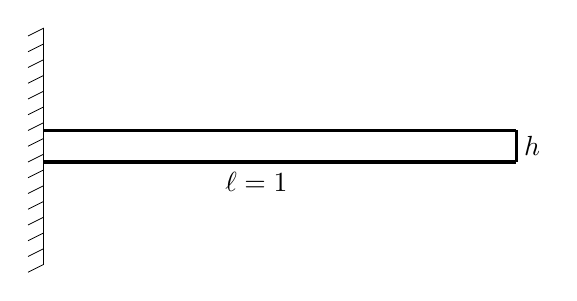
\begin{tikzpicture}
						\draw[line width = 0.4mm] (0,0.2) -- (6,0.2);
						\draw[line width = 0.4mm] (0,-0.2) -- (6,-0.2);
						\draw[line width = 0.4mm] (6,-0.2) -- (6,0.2);
						%\draw[line width = 0.4mm] (0,-0.2) -- (0,0.2);
						
						%\draw[line width = 0.1mm,->] (6,2) -- (7.4,2);
						%\draw[line width = 0.1mm,->] (6,2) -- (6,0.9);
						%\node at (6.7,1.8) {$e_1$};
						%\node at (5.8,1.4) {$e_2$};
						
						\node at (6.2,0) {$h$};
						\node at (2.7,-0.45) {$\ell = 1$};
						
						\draw[line width = 0.1mm] (0,-1.5) -- (0,1.5);
						\draw[line width = 0.1mm] (0,1.5) -- (-0.2,1.4);
						\draw[line width = 0.1mm] (0,1.3) -- (-0.2,1.2);
						\draw[line width = 0.1mm] (0,1.1) -- (-0.2,1);
						\draw[line width = 0.1mm] (0,0.9) -- (-0.2,0.8);
						\draw[line width = 0.1mm] (0,0.7) -- (-0.2,0.6);
						\draw[line width = 0.1mm] (0,0.5) -- (-0.2,0.4);
						\draw[line width = 0.1mm] (0,0.3) -- (-0.2,0.2);
						\draw[line width = 0.1mm] (0,0.1) -- (-0.2,0);
						
						\draw[line width = 0.1mm] (0,-0.1) -- (-0.2,-0.2);
						\draw[line width = 0.1mm] (0,-0.3) -- (-0.2,-0.4);
						\draw[line width = 0.1mm] (0,-0.5) -- (-0.2,-0.6);
						\draw[line width = 0.1mm] (0,-0.7) -- (-0.2,-0.8);
						\draw[line width = 0.1mm] (0,-0.9) -- (-0.2,-1);
						\draw[line width = 0.1mm] (0,-1.1) -- (-0.2,-1.2);
						\draw[line width = 0.1mm] (0,-1.3) -- (-0.2,-1.4);
						\draw[line width = 0.1mm] (0,-1.5) -- (-0.2,-1.6);
						
						%\node at (3.2,-0.3) {$\ell = 1$};
					
					\end{tikzpicture}
				\end{center}
				\subcaption{Two-Dimensional Cantilever Beam}
			\end{minipage}
		}
	}
\end{figure}\label{fig:compare:1D+2D}

In the derivation of the Timoshenko beam model in Section \ref{subsec:equationsofmotion+constitutiveequation}, the parameter $\alpha$ is 
introduced. The paramater is given here again for convenience:
\begin{eqnarray*}
	\alpha = \frac{A\ell^2}{I}.
\end{eqnarray*}

The model is in a dimensionless form, therefore the length of the beam is $\ell = 1$. Since we assumed a square cross-section, the area of the cross-section can be calculated as $\displaystyle A = hb$. The area moment of inertia can also be calculated as $\displaystyle I = \frac{h^3b}{12}$. Substituting these values into the formula for $\alpha$ gives the following relationship between the height of the beam and the parameter $\alpha$: $\displaystyle \alpha = \frac{12}{h^2}$
or equivalently,
\begin{eqnarray}
	h & = & \sqrt{\frac{12}{\alpha}}. \label{eq:h-alpha-relationship}
\end{eqnarray}
 Using this relationship, the height of the beam model can be set by considering the value of $\alpha$.


\subsection{Calculating the eigenvalues and eigenvectors}
In Section \ref{sec:Timo:EigenvalueProblem} a method for calculating the eigenvalues and eigenvectors of the Timoshenko beam is provided. And in Section \ref{sec:Timo:Cantilever}, the eigenvalues and eigenvectors of a cantilever Timoshenko beam are calculated as an example. 

For the two-dimensional beam, the eigenvalues and eigenvectors are calculated using the Finite Element Method. In Section \ref{sec:FEM:2D}, the Finite Element Method for a cantilever two-dimensional beam is derived. Specifically, Section \ref{2dFEM_EP} derives the eigenvalue problem for the two-dimensional beam using the Finite Element Method, called Problem 2D-1E.

\subsubsection{Problem 2D-1E}
Find a real number $\lambda$ and a vector $\bar{u} \in R^n$ such that
\begin{eqnarray}
	K\bar{u} & = & M\lambda{\bar{u}},
\end{eqnarray} where $M$ and $K$ are the standard Finite Element Method matrices defined in Section \ref{sec:FEM:2D}.

In this form, the eigenvalue problem is a system of ordinary differential equations, and can be solved using a numerical method. Computer programs like MATLAB provide functions that are able to solve this.

\subsubsection{Accuracy of the eigenvalues}
Solving \textbf{Problem 2D-1E} with a numerical method, requires a quick investigation into the rate of convergence so that the accuracy of the eigenvalues can be established. Chapter \ref{ch:finite-element-theory} provides the necessary theory on the existence of solutions as well as the proof of convergence of the Finite Element Method.

\begin{figure}[H]
    \centering
    \begin{adjustbox}{center}
        \includegraphics[scale=0.7]{Convergence.png}
    \end{adjustbox}
    \caption{Rate of convergence of the first 20 eigenvalues.}
    \label{fig:conv_2d_eig}
\end{figure}


Figure \ref{fig:conv_2d_eig} shows the rate of convergence of the first 20 eigenvalues of the two-dimensional beam. Each color represents a spesific eigenvalue.

The number of elements are chosen so that at least the first 10 eigenvalues are accurate to 5 significant digits.

\subsection{Comparing the mode shapes}
Recall from the introduction, that the investigation is focussed on beam-type problems. The two-dimensional model is for an eigenvalue problem and and not specific to beam-type applications, like the Timoshenko beam model. Therefore there are non-beam type modes that can be expected from the two-dimensional model. This is also be reflected in the eigenvalues of the two-dimensional model and therefore eigenvalues irrelevant to beam-type problems exits.

Therefore a method is required to compare and match the eigenvalues of the two models. In \cite{LVV09}, the authors compare the mode shapes of the two models, to match up the eigenvalues. Eigenvalues relating to the mode shapes similar to the mode shapes of the Timoshenko beam, are called beam-type eigenvalues. The other eigenvalues are called non-beam type eigenvalues by the authors.

\subsubsection{Shapes relating to beam-type eigenvalues}
The following figures are examples of beam-type mode shapes for the displacement $w$.

\begin{figure}[h!]
	\scalebox{.8}{
		\makebox[\textwidth][c]{
			\centering
			\begin{minipage}[b]{0.8\linewidth}
				\includegraphics[width=1\linewidth]{Beam1.jpg}
				\subcaption{2D Beam Type - $\lambda_6 = 21.911$}
				\label{fig:minipage2}
			\end{minipage}
			\begin{minipage}[b]{0.8\linewidth}
				\includegraphics[width=1\linewidth]{1DBeam2.png}
				\subcaption{Timoshenko - $\lambda_5 = 21.794$}
				\label{fig:minipage1}
			\end{minipage}
	}}
	\scalebox{.8}{
		\makebox[\textwidth][c]{
			\begin{minipage}[b]{0.8\linewidth}
				\includegraphics[width=1\linewidth]{Beam2.jpg}
				\subcaption{2D Beam Type - $\lambda_7 = 45.711$}
				\label{fig:minipage2}
			\end{minipage}
			\begin{minipage}[b]{0.8\linewidth}
				\includegraphics[width=1\linewidth]{1DBeam1.png}
				\subcaption{Timoshenko - $\lambda_6 = 45.390$}
				\label{fig:minipage1}
			\end{minipage}
			\caption{Modal shapes of the displacement $w$ for the beam-type 2D body and the Timoshenko beam with $\alpha = 4800$ ($h = 1/20$).}
		}
	}
\end{figure}
\FloatBarrier

\subsubsection{Shapes relating to non-beam type eigenvalues}
The following figures are examples of non beam-type mode shapes for the displacement $w$. These mode shapes are not present in the cantilever Timoshenko beam model and are not beam related. 
\begin{figure}[h!]
	\scalebox{.8}{
		\makebox[\textwidth][c]{
			\centering
			\begin{minipage}[b]{0.8\linewidth}
				\includegraphics[width=1\linewidth]{NotBeam1.jpg}
				\subcaption{Non-Beam Type - $\lambda_4 = 7.7077$}
				\label{fig:minipage2}
			\end{minipage}
			\begin{minipage}[b]{0.8\linewidth}
				\includegraphics[width=1\linewidth]{NotBeam2.jpg}
				\subcaption{Non-Beam Type - $\lambda_8 = 69.344$}
				\label{fig:minipage1}
			\end{minipage}
			\caption{Modal shapes of the displacement $w$ for the non-beam type 2D body with $h = 1/20$.}
		}
	}
\end{figure}
\FloatBarrier

\subsubsection{Shape of the cross-sections}
The Timoshenko beam theory improve some one-dimensional beam theories such as the Euler-Bernoulli beam theory by also including the effect of shear. For Timoshenko beam theory it is assumed that the cross-sections need not remain perpendicular to the neutral axis of the beam. The cross-sections however remain a straight line.

For the two-dimensional beam, the shape of the cross-section can deform into a S-shape. This is explained in \cite{LVV09} and a similar figure in \cite{LVV09} is given here. 

\FloatBarrier
\begin{figure}[h!]
	\centering
	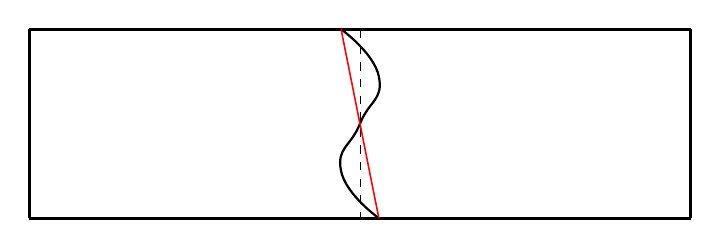
\begin{tikzpicture}[scale=1.2]
	
	\draw[line width = 0.4mm] (0,1) -- (7,1);
	\draw[line width = 0.4mm] (0,-1) -- (7,-1);
	\draw[line width = 0.4mm] (7,-1) -- (7,1);
	\draw[line width = 0.4mm] (0,-1) -- (0,1);
	
	
	\draw[line width = 0.1mm,dashed] (3.5,1) -- (3.5,-1);
	
	\draw[thick] plot [smooth,tension=0.9] coordinates{(3.3,1) (3.7,0.5) (3.5,0) (3.3,-0.5) (3.7,-1)};
	
	\draw[line width = 0.2mm,red] (3.3,1) -- (3.7,-1);
	
\end{tikzpicture}
	\caption{S-shape deformation of the cross-section of the two-dimensional beam.}\label{fig:s}
\end{figure}
\FloatBarrier

Note that figure \ref{fig:s} shows an exaggerated example of the deformation of a cross-section. The red line shows how the authors of \cite{LVV09} calculated the average rotation of a cross-section of the two-dimensional beam. This average rotation can be used to compare the rotation of the cross-section of the two-dimensional beam to the rotation of the cross-section of the Timoshenko beam given by $\phi$.

\subsubsection{Direct comparison of mode shapes}
Figure \ref{fig:w} directly compares a mode shape of the Timoshenko beam to a mode shape of the two-dimensional beam. For the two-dimensional model, the center line of the displacement of the beam is shown. For the Timoshenko beam, the displacement $w$ is shown.

\begin{figure}[ht!]
	\scalebox{.8}{
		\makebox[\textwidth]{
			\centering
			\centering
			\includegraphics[scale=0.4]{1Dv2D.png}
			\caption{Comparison of the displacement $w$ mode shape corresponding to $\lambda_{10}$ for the 2D beam and $\lambda_8$ for the Timoshenko beam with $\alpha = 4800$ ($h=1/20$)}
			\label{fig:w}}}
\end{figure}
\FloatBarrier

Similarly, figure \ref{fig:phi} directly compares the angle of the cross-section of the Timoshenko beam and the two-dimensional beam. The average rotation of the cross-section of the two-dimensional beam's mode shape is calculated as shown in figure \ref{fig:s}.

\FloatBarrier
\begin{figure}[ht!]
	\scalebox{.8}{
		\makebox[\textwidth]{
			\centering
			\centering
			\includegraphics[scale=0.4]{1Dv2Dphi.png}
			\caption{Comparison of the angle $\phi$ (best fit for 2D Beam) mode shape corresponding to $\lambda_{10}$ for the 2D beam and $\lambda_8$ for the Timoshenko beam with $\alpha = 4800$ ($h=1/20$)}
			\label{fig:phi}}}
\end{figure}
\FloatBarrier

These figures are examples that show how similar the mode shapes of the two models are. This specific example is for $\alpha = 4800$, which represents a typical beam. The authors of \cite{LVV09} obtained similar results for $\alpha=300$, which represents a short and thick beam.

\textbf{Remark:} Note that the overall shape is important. This is because any multiple of a eigenvector is still an eigenvector. The mode shapes were specifically scaled to obtain figures \ref{fig:w} and \ref{fig:phi}.

\subsection{Comparing the eigenvalues}
Using this method of comparing the mode shapes, the eigenvalues can now be matched up and compared. In the tables, Timo refers to the Timoshenko beam and 2D refers to the two-dimensional beam.

\subsubsection{Some results from [LVV09]}
The following table contains results from \cite{LVV09} verbatim to 3 significant digits, as well as the replicated results to 5 significant digits.



\begin{table}[!ht]
	\centering
	\caption{Results from [LVV09] and results obtained in this dissertation. $0^*$ indicates a 0 as a result of rounding. $\alpha = 1200$.}
	\begin{tabular}{|c|c|c||c|c|c|}
		\hline
		\multicolumn{3}{|c||}{Results from [LVV09]} & \multicolumn{3}{c|}{Dissertation} \\ \hline \hline
		~ & 2D & Timo & ~ & 2D & Timo  \\ \hline
		1 & 0.0317 & 0.0316 & 1 & 0.031713 & 0.031639  \\ 
		2 & 1.14 & 1.14  & 2 & 1.1413 & 1.1365  \\ 
		3 & 7.72 & - & 3 & 7.7161 & - \\ 
		4 & 7.92 & 7.86 &  4 & 7.918 & 7.8617    \\ 
		5 & 26.2 & 25.9 & 5 & 26.148 & 25.869   \\ 
		6 & 60.8 & 59.9 & 6 & 60.816 & 59.946  \\ 
		7 & 69.3 & - & 7 & 69.344 & -  \\ 
		8 & 115 & 113 &  8 & 115.28 & 113.23   \\ 
		9 & 192 & 188 &  9 & 191.57 & 187.55   \\ 
		10 & 192 & - & 10 & 192.03 & -  \\ 
		11 & 291 & 284 & 11 & 290.76 & 283.81   \\ \hline
	\end{tabular}\label{Results_LVV09}
\end{table}


\begin{comment}
\begin{table}[!ht]
	\centering
	\caption{Results from [LVV09] and results obtained in this dissertation. $0^*$ indicates a 0 as a result of rounding. $\alpha = 1200$.}
	\begin{tabular}{|c|c|c|c||c|c|c|c|}
		\hline
		\multicolumn{4}{|c||}{Results from [LVV09]} & \multicolumn{4}{c|}{Dissertation} \\ \hline \hline
		~ & 2D & Timo & RE & ~ & 2D & Timo & RE  \\ \hline
		1 & 0.0317 & 0.0316 & 0.00315 & 1 & 0.031713 & 0.031639 & 0.0023407  \\ 
		2 & 1.14 & 1.14 & $0^*$ & 2 & 1.1413 & 1.1365 &  0.0042050 \\ 
		3 & 7.72 & - & ~ & 3 & 7.7161 & - &   \\ 
		4 & 7.92 & 7.86 & 0.00758 & 4 & 7.918 & 7.8617 & 0.0071116    \\ 
		5 & 26.2 & 25.9 & 0.0115 & 5 & 26.148 & 25.869 & 0.010669  \\ 
		6 & 60.8 & 59.9 & 0.0148 & 6 & 60.816 & 59.946 & 0.014303  \\ 
		7 & 69.3 & - & ~ & 7 & 69.344 & - &    \\ 
		8 & 115 & 113 & 0.0174 & 8 & 115.28 & 113.23 &  0.017787  \\ 
		9 & 192 & 188 & 0.0208 & 9 & 191.57 & 187.55 &  0.020999  \\ 
		10 & 192 & - &  & 10 & 192.03 & - &   \\ 
		11 & 291 & 284 & 0.0241 & 11 & 290.76 & 283.81 &  0.023899  \\ \hline
	\end{tabular}\label{Results_LVV09}
\end{table}
\end{comment}


This table shows that the results obtained in this dissertation are very similar to the results obtained in \cite{LVV09}. This is for a specific case where $\alpha = 1200$.

In the following table, the eigenvalues for different values of $\alpha$ are compared.

\begin{table}[h!]
	\scalebox{.8}{
	\makebox[\textwidth]{
	\caption{Eigenvalues of a Timoshenko cantilever beam vs the eigenvalues of a cantilever two-dimensional elastic body. *RE is the relative error.}
	\begin{tabular}{|cccc||cccc||cccc||cccc|}
		\hline
		\multicolumn{16}{|c|}{Comparison of Eigenvalues} \\
		\hline\hline
		\multicolumn{4}{|c||}{ $h = 1/5$ or $\alpha = 300$}       & \multicolumn{4}{c||}{$h =1/10$ or $\alpha = 1200$}      & \multicolumn{4}{c||}{$h = 1/20$ or $\alpha = 4800$}      & \multicolumn{4}{c|}{$h = 1/30$ or $\alpha = 10800$} \\
		\hline
		{i} & {2D} & {j} & {Timo} & {i} & {2D} & {j} & {Timo} & {i} & {2D} & {j} & {Timo} & {i} & {2D} & {j} & {Timo} \\
		\hline
		{1}&0.12151&1&0.12092&1&0.031713&1&0.031639&1&0.008013&1&0.008004&1&0.003568&1&0.003565\\
		{2}&3.5460&2&3.5071&2&1.1413&2     & 1.1365 & 2     & 0.30756 & 2     & 0.30705 & 2     & 0.13869 & 2     & 0.13855 \\
		\cellcolor{lightgray}{3} & \cellcolor{lightgray}{7.7311} &       & {-} & \cellcolor{lightgray}{3}     & \cellcolor{lightgray}{7.7161} &       & {-} & 3     & 2.3273 & 3     & 2.3213 & 3     & 1.0698 & 3     & 1.0683 \\
		{4} & 20.225 & 3     & 19.869 & 4     & 7.9180 & 3     & 7.8617 & \cellcolor{lightgray}{4}     & \cellcolor{lightgray}{7.7077} &       & {-} & 4     & 4.0140 & 4     & 4.0058 \\
		{5} & 56.109 & 4     & 54.766 & 5     & 26.148 & 4     & 25.869 & 5     & 8.5086 & 4     & 8.4762 & \cellcolor{lightgray}{5}     & \cellcolor{lightgray}{7.7047} &       & {-} \\
		\cellcolor{lightgray}{6} & \cellcolor{lightgray}{69.164} &       & {-} & 6     & 60.816 & 5     & 59.946 & 6     & 21.911 & 5     & 21.794 & 6     & 10.655 & 5     & 10.625 \\
		{7} & 114.03 & 5     & 110.75 & \cellcolor{lightgray}{7}     & \cellcolor{lightgray}{69.344} &       & {-} & 7     & 45.711 & 6     & 45.390 & 7     & 22.975 & 6     & 22.890 \\
		{8} & {189.17} &  6     & {186.50} & 8     & 115.28 & 6     & 113.23 & \cellcolor{lightgray}{8}     & \cellcolor{lightgray}{69.344} &       & {-} & 8     & 43.113 & 7     & 42.909 \\
		\cellcolor{lightgray}{9} & \cellcolor{lightgray}{192.61} &      &  & {9}     & {191.57} &   7  & {187.55} & 9     & 82.887 & 7     & 82.154 & \cellcolor{lightgray}{9}     & \cellcolor{lightgray}{69.331} &       & {-} \\
		{10} & 285.85 & 7     & 277.64 & \cellcolor{lightgray}{10}    & \cellcolor{lightgray}{192.03} &      & {-} & 10    & 136.03 & 8     & 134.58 & 10    & 73.230 & 8     & 72.803 \\
		{11} & 328.40 & 8     & 330.29 & 11    & 290.76 & 8     & 283.81 & \cellcolor{lightgray}{11}    & \cellcolor{lightgray}{192.48} &       & {-} & 11    & 115.41 & 9     & 114.61 \\
		\cellcolor{lightgray}{12} & \cellcolor{lightgray}{357.08} &       & {-} & \cellcolor{lightgray}{12}    & \cellcolor{lightgray}{374.45} &       & {-} & 12    & 207.29 & 9     & 204.69 & 12    & 171.61 & 10    & 170.20 \\
		{13} & 397.33 & 9     & 394.02 & 13    & 413.20 & 9     & 402.27 & 13    & 298.38 & 10    & 294.10 & \cellcolor{lightgray}{13}    & \cellcolor{lightgray}{192.52} &       & {-} \\
		{14} & 442.00   & 10    & 439.52 & 14    & 558.67 & 10    & 542.65 & \cellcolor{lightgray}{14}    & \cellcolor{lightgray}{376.83} &       & {-} & 14    & 243.56 & 11    & 241.26 \\
		\cellcolor{lightgray}{15} & \cellcolor{lightgray}{533.71} &       & {-} & \cellcolor{lightgray}{15}    & \cellcolor{lightgray}{614.11} &       & {-} & 15    & 410.63 & 11    & 404.01 & 15    & 332.83 & 12    & 329.28 \\
		{16} & 538.97 & 11    & 541.55 & 16    & 726.26 & 11    & 704.15 & 16    & 545.03 & 12    & 535.32 & \cellcolor{lightgray}{16}    & \cellcolor{lightgray}{377.16} &       & {-} \\
		\cellcolor{lightgray}{17} & \cellcolor{lightgray}{596.06} &       & {-} & \cellcolor{lightgray}{17}    & \cellcolor{lightgray}{906.28} &       & {-} & \cellcolor{lightgray}{17}    & \cellcolor{lightgray}{621.95} &       & {-} & 17    & 440.77 & 13    & 435.51 \\
		{18} & 602.77 & 12    & 596.09 & 18    & 913.69 & 12    & 884.92 & 18    & 702.30 & 13    & 688.64 & 18    & 568.51 & 14    & 561.04 \\
		\cellcolor{lightgray}{19} & \cellcolor{lightgray}{657.87} &       & {-} & 19    & 1113.7 & 13    & 1080.1 & 19    & 882.95 & 14    & 864.40 & \cellcolor{lightgray}{19}    & \cellcolor{lightgray}{623.05} &       & {-} \\
		{20} & 717.37 & 13    & 731.74 & \cellcolor{lightgray}{20}    & \cellcolor{lightgray}{1218.0}  &       & {-} & \cellcolor{lightgray}{20}    & \cellcolor{lightgray}{927.18} &       & {-} & 20    & 717.04 & 15    & 706.74 \\
		\hline
		\multicolumn{2}{|c}{Max RE:} & \multicolumn{2}{c||}{3.1718\%} & \multicolumn{2}{c}{Max RE:} & \multicolumn{2}{c||}{3.1486\%} & \multicolumn{2}{c}{Max RE:} & \multicolumn{2}{c||}{2.1018\%} & \multicolumn{2}{c}{Max RE:} & \multicolumn{2}{c|}{1.4361\%} \\
		\hline
	\end{tabular}%
	\label{tab:Timo}%
}
}
\end{table}%
\FloatBarrier

This table shows that the eigenvalues of the Timoshenko model and the two-dimensional model compare very well. The non-beam type eigenvalues are highlighted in grey. For a short thick beam ($\alpha = 300$), the maximum relative error for the first 20 two-dimensional eigenvalues is just over $3\%$, while for a long thin beam ($\alpha = 10800$), the maximum relative error is just over $1\%$. This shows that as the beam becomes longer and thinner, the Timoshenko beam is a better approximation of the two-dimensional beam. But overall the Timoshenko beam compares very well.

This table also shows that as the beam gets more narrow, there are less non-beam type eigenvalues within the first few eigenvalues.This would also indicate that the Timoshenko beam would be a better approximation of the two-dimensional beam as the beam gets more narrow since the two-dimensional model behaves `more like a beam'.


\end{document}